\documentclass[../../../analisi-dei-requisiti.tex]{subfiles}

\begin{document}

\subsubsection{AUC10: Eliminazione owner}%
\label{subs:AUC10}

\begin{figure}[H]
  \centering
  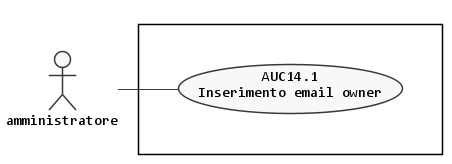
\includegraphics[width=100mm]{eliminazione-owner.png}
  \caption{AUC10: Eliminazione owner}%
  \label{fig:AUC10}
\end{figure}

\begin{description}
  \item[Codice:] AUC10;
  \item[Titolo:] Eliminazione owner;
  \item[Attori primari:] amministratore;
  \item[Precondizione:] il sistema deve rendere disponibile la pagina di eliminazione owner;
  \item[Postcondizione:] l'utente non è più owner;
  \item[Scenario principale:]
  \begin{enumerate}
    \item l'amministratore vuole eliminare i privilegi ad un utente owner.
  \end{enumerate}
\end{description}

\subsubsection{AUC10.1: Inserimento email owner}%
\label{subs:AUC10.1}
\begin{description}
  \item[Codice:] AUC10.1;
  \item[Titolo:] Inserimento email owner;
  \item[Attori primari:] amministratore;
  \item[Precondizione:] il sistema deve rendere disponibile la possibilità di inserire l'email dell'owner da eliminare;
  \item[Postcondizione:] l'email viene opportunemente inserita;
  \item[Scenario principale:]
  \begin{enumerate}
    \item l'amministratore inserisce l'email dell'owner da eliminare.
  \end{enumerate}
\end{description}

\end{document}
